% !TeX root = ../Report.tex

% ساختار کار، یافته‌ها، تئوری‌ها ، (توصیفی، فرضیات،  آزمون‌ها) |تحلیل و طراحی سیستم


\addcontentsline{toc}{section}{مقدمه}
\section*{مقدمه}
در این فصل به نحوه طراحی و پیاده سازی نرم‌افزار پرداخته شده است.
\begin{figure}[H]
	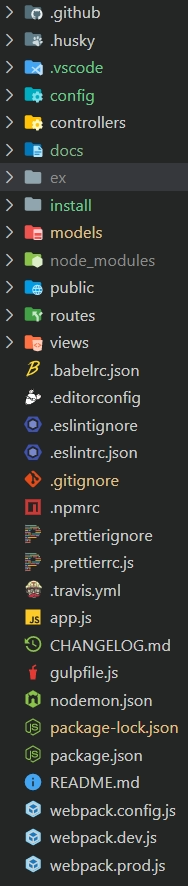
\includegraphics[width=.3\textwidth]{Folders-Files/all.png}
	\centering
	\caption{ساختار کلی}
	\label{fig:folder-main}
\end{figure}

\section{پوشه تنظیمات (config)}
در این پوشه تنظیمات نرم‌افزار قرار دارد. 

\begin{figure}[H]
	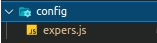
\includegraphics[width=.3\textwidth]{Folders-Files/config.png}
	\centering
	\caption{ساختار پوشه تنظیمات}
	\label{fig:folder-config}
\end{figure}

\paragraph{فایل expers}
در این فایل به تنظیمات فریم‌ورک اکسپرس که شامل ارتباط با پایگاه داده و فراخوانی فایل‌های .env و package پرداخته شده است. 

\paragraph{\rl{logInChecker}:}
اعتبارسنجی ورود کاربر به سایت.
\\
\textbf{توضیحات}
\hr
\begin{flushleft}
	\framebox[.9\textwidth][l]{
		\lr{
			\textcolor{type}{void}
			\textcolor{func}{logInChecker}
			\textcolor{symb}{(}
			\textcolor{type}{object}
			\textcolor{arg}{request}
			\textcolor{symb}{,}
			\textcolor{type}{object}
			\textcolor{arg}{response}
			\textcolor{symb}{,}
			\textcolor{type}{object}
			\textcolor{arg}{next}
			\textcolor{symb}{);}
		}
	}
\end{flushleft}
بررسی طلاعات کاربری و اعتبار زمانی.
\\
\textbf{پارامترها}
\hr \\[10pt]
\begin{tabular}{|m{4cm}|m{3cm}|m{10cm}|}
	\hline
	\multicolumn{1}{|c}{پارامتر}
	&
	\multicolumn{1}{|c}{نوع}
	&
	\multicolumn{1}{|c|}{توضیحات}
	\\
	\hline
	\multicolumn{1}{|c}{request}
	&
	\multicolumn{1}{|c|}{object}
	&
	نمایانگر درخواست HTTP و دارای خصوصیاتی برای درخواست رشته پرس‌و‌جو، پارامترها ، بدنه ، هدرهای HTTP و غیره است.
	در این اسناد و طبق قرارداد ، از این شی همیشه به عنوان req یاد می شود (و پاسخ HTTP res است).
	\\
	\hline
	\multicolumn{1}{|c}{response}
	&
	\multicolumn{1}{|c|}{object}
	&
	نمایانگر پاسخ HTTP که برنامه Express با دریافت درخواست HTTP ارسال می کند.
	در این اسناد و طبق قرارداد ، از شی همیشه به عنوان res یاد می شود (و درخواست HTTP req است).
	\\
	\hline
	\multicolumn{1}{|c}{next}
	&
	\multicolumn{1}{|c|}{object}
	&
	عملکرد میان‌افزار بعدی را نشان می دهد.
	\\
	\hline
\end{tabular}
\\[10pt]
\textbf{خروجی}
\hr \\
در صورتی که کاربر به سایت وارد شده باشد یا مهلت زمانی ورود کاربر به پایان نرسیده باشد برنامه ادامه می‌یابد، در غیر این صورت به صفحه ورود به سایت هدایت می‌شود.


\section{پوشه کنترل (controllers)}
% !TeX root = ../../Report.tex
% !TeX encoding = UTF-8

در این قسمت تمام عملیات‌های پردازش درخواست‌ها شامل ثبت، ویرایش و ... کنترل می‌شوند.

\begin{figure}[H]
	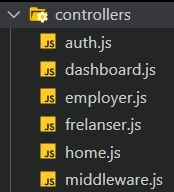
\includegraphics[width=.3\textwidth]{Folders-Files/controllers.png}
	\centering
	\caption{ساختار پوشه کنترل}
	\label{fig:folder:controllers}
\end{figure}

\subsection{فایل middleware}
در این فایل به میان‌افزارهای کنترل‌ مانند کنترل سطح دسترسی کاربر، کنترل ورود کاربر و ... پرداخته شده است.

\paragraph{\rl{logInChecker}:}
اعتبارسنجی ورود کاربر.
\\
\textbf{توضیحات}
\hr
\begin{flushleft}
	\framebox[.9\textwidth][l]{
		\lr{
			\textcolor{type}{void}
			\textcolor{func}{logInChecker}
			\textcolor{symb}{(}
			\textcolor{type}{object}
			\textcolor{arg}{request}
			\textcolor{symb}{,}
			\textcolor{type}{object}
			\textcolor{arg}{response}
			\textcolor{symb}{,}
			\textcolor{type}{object}
			\textcolor{arg}{next}
			\textcolor{symb}{);}
		}
	}
\end{flushleft}
در صورتی که کاربر به سایت وارد شده باشد، برنامه ادامه می‌یابد، در غیر این صورت به صفحه ورود به سایت هدایت می‌شود.
\\
\textbf{پارامترها}
\hr \\[10pt]
\begin{tabular}{|m{4cm}|m{3cm}|m{10cm}|}
	\hline
	\multicolumn{1}{|c}{پارامتر}
	&
	\multicolumn{1}{|c}{نوع}
	&
	\multicolumn{1}{|c|}{توضیحات}
	\\
	\hline
	\multicolumn{1}{|c}{request}
	&
	\multicolumn{1}{|c|}{object}
	&
	نمایانگر درخواست HTTP و دارای خصوصیاتی برای درخواست رشته پرس‌و‌جو، پارامترها ، بدنه ، هدرهای HTTP و غیره است.
	در این اسناد و طبق قرارداد ، از این شی همیشه به عنوان req یاد می شود (و پاسخ \lr{HTTP res} است).
	\\
	\hline
	\multicolumn{1}{|c}{response}
	&
	\multicolumn{1}{|c|}{object}
	&
	نمایانگر پاسخ HTTP که برنامه Express با دریافت درخواست HTTP ارسال می کند.
	در این اسناد و طبق قرارداد ، از شی همیشه به عنوان res یاد می شود (و درخواست \lr{HTTP req} است).
	\\
	\hline
	\multicolumn{1}{|c}{next}
	&
	\multicolumn{1}{|c|}{object}
	&
 میان‌افزار بعدی را اجرا می‌کند.
	\\
	\hline
\end{tabular}
\\[10pt]
\textbf{خروجی}
\hr \\
ندارد.

\paragraph{\rl{sessionChecker}:}
اعتبارسنجی نشست‌های برنامه.
\\
\textbf{توضیحات}
\hr
\begin{flushleft}
	\framebox[.9\textwidth][l]{
		\lr{
			\textcolor{type}{void}
			\textcolor{func}{sessionChecker}
			\textcolor{symb}{(}
			\textcolor{type}{object}
			\textcolor{arg}{request}
			\textcolor{symb}{,}
			\textcolor{type}{object}
			\textcolor{arg}{response}
			\textcolor{symb}{,}
			\textcolor{type}{object}
			\textcolor{arg}{next}
			\textcolor{symb}{);}
		}
	}
\end{flushleft}
در صورتی که مهلت زمانی ورود کاربر به پایان نرسیده باشد برنامه ادامه می‌یابد، در غیر این صورت به صفحه ورود به سایت هدایت می‌شود.
\\
\textbf{پارامترها}
\hr \\[10pt]
\begin{tabular}{|m{4cm}|m{3cm}|m{10cm}|}
	\hline
	\multicolumn{1}{|c}{پارامتر}
	&
	\multicolumn{1}{|c}{نوع}
	&
	\multicolumn{1}{|c|}{توضیحات}
	\\
	\hline
	\multicolumn{1}{|c}{request}
	&
	\multicolumn{1}{|c|}{object}
	&
	نمایانگر درخواست HTTP و دارای خصوصیاتی برای درخواست رشته پرس‌و‌جو، پارامترها ، بدنه ، هدرهای HTTP و غیره است.
	در این اسناد و طبق قرارداد ، از این شی همیشه به عنوان req یاد می شود (و پاسخ \lr{HTTP res} است).
	\\
	\hline
	\multicolumn{1}{|c}{response}
	&
	\multicolumn{1}{|c|}{object}
	&
	نمایانگر پاسخ HTTP که برنامه Express با دریافت درخواست HTTP ارسال می کند.
	در این اسناد و طبق قرارداد ، از شی همیشه به عنوان res یاد می شود (و درخواست \lr{HTTP req} است).
	\\
	\hline
	\multicolumn{1}{|c}{next}
	&
	\multicolumn{1}{|c|}{object}
	&
 میان‌افزار بعدی را اجرا می‌کند.
	\\
	\hline
\end{tabular}
\\[10pt]
\textbf{خروجی}
\hr \\
ندارد.

\paragraph{\rl{roleChecker}:}
اعتبارسنجی سطح دسترسی کاربر به محتوا.
\\
\textbf{توضیحات}
\hr
\begin{flushleft}
	\framebox[.9\textwidth][l]{
		\lr{
			\textcolor{type}{void}
			\textcolor{func}{logInChecker}
			\textcolor{symb}{(}
			\textcolor{type}{object}
			\textcolor{arg}{request}
			\textcolor{symb}{,}
			\textcolor{type}{object}
			\textcolor{arg}{response}
			\textcolor{symb}{,}
			\textcolor{type}{object}
			\textcolor{arg}{next}
			\textcolor{symb}{);}
		}
	}
\end{flushleft}
در صورتی که سطح دسترسی کاربر مجار باشد برنامه ادامه می‌یابد، در غیر این صورت به صفحه قبل از درخواست هدایت می‌شود.
\\
\textbf{پارامترها}
\hr \\[10pt]
\begin{tabular}{|m{4cm}|m{3cm}|m{10cm}|}
	\hline
	\multicolumn{1}{|c}{پارامتر}
	&
	\multicolumn{1}{|c}{نوع}
	&
	\multicolumn{1}{|c|}{توضیحات}
	\\
	\hline
	\multicolumn{1}{|c}{request}
	&
	\multicolumn{1}{|c|}{object}
	&
	نمایانگر درخواست HTTP و دارای خصوصیاتی برای درخواست رشته پرس‌و‌جو، پارامترها ، بدنه ، هدرهای HTTP و غیره است.
	در این اسناد و طبق قرارداد ، از این شی همیشه به عنوان req یاد می شود (و پاسخ \lr{HTTP res} است).
	\\
	\hline
	\multicolumn{1}{|c}{response}
	&
	\multicolumn{1}{|c|}{object}
	&
	نمایانگر پاسخ HTTP که برنامه Express با دریافت درخواست HTTP ارسال می کند.
	در این اسناد و طبق قرارداد ، از شی همیشه به عنوان res یاد می شود (و درخواست \lr{HTTP req} است).
	\\
	\hline
	\multicolumn{1}{|c}{next}
	&
	\multicolumn{1}{|c|}{object}
	&
 میان‌افزار بعدی را اجرا می‌کند.
	\\
	\hline
\end{tabular}
\\[10pt]
\textbf{خروجی}
\hr \\
ندارد.

\subsection{فایل auth}
در این فایل به کنترل عملیات‌های احرازهویت پرداخته شده است.

\paragraph{\rl{getRegister}:}
اطلاعات صفحه ثبت‌نام را بارگذاری می‌کند.
\\
\textbf{توضیحات}
\hr
\begin{flushleft}
	\framebox[.9\textwidth][l]{
		\lr{
			\textcolor{type}{void}
			\textcolor{func}{getRegister}
			\textcolor{symb}{(}
			\textcolor{type}{object}
			\textcolor{arg}{request}
			\textcolor{symb}{,}
			\textcolor{type}{object}
			\textcolor{arg}{response}
			\textcolor{symb}{);}
		}
	}
\end{flushleft}
بارگذاری اطلاعات صفحه ثبت‌نام کاربر. 
\\
\textbf{پارامترها}
\hr \\[10pt]
\begin{tabular}{|m{4cm}|m{3cm}|m{10cm}|}
	\hline
	\multicolumn{1}{|c}{پارامتر}
	&
	\multicolumn{1}{|c}{نوع}
	&
	\multicolumn{1}{|c|}{توضیحات}
	\\
	\hline
	\multicolumn{1}{|c}{request}
	&
	\multicolumn{1}{|c|}{object}
	&
	نمایانگر درخواست HTTP و دارای خصوصیاتی برای درخواست رشته پرس‌و‌جو، پارامترها ، بدنه ، هدرهای HTTP و غیره است.
	در این اسناد و طبق قرارداد ، از این شی همیشه به عنوان req یاد می شود (و پاسخ \lr{HTTP res} است).
	\\
	\hline
	\multicolumn{1}{|c}{response}
	&
	\multicolumn{1}{|c|}{object}
	&
	نمایانگر پاسخ HTTP که برنامه Express با دریافت درخواست HTTP ارسال می کند.
	در این اسناد و طبق قرارداد ، از شی همیشه به عنوان res یاد می شود (و درخواست \lr{HTTP req} است).
	\\
	\hline
\end{tabular}
\\[10pt]
\textbf{خروجی}
\hr \\
ندارد.

\paragraph{\rl{postRegister}:}
ثبت اطلاعات کاربر در بانک اطلاعات
\\
\textbf{توضیحات}
\hr
\begin{flushleft}
	\framebox[.9\textwidth][l]{
		\lr{
			\textcolor{type}{void}
			\textcolor{func}{postRegister}
			\textcolor{symb}{(}
			\textcolor{type}{object}
			\textcolor{arg}{request}
			\textcolor{symb}{,}
			\textcolor{type}{object}
			\textcolor{arg}{response}
			\textcolor{symb}{);}
		}
	}
\end{flushleft}
ثبت اطلاعات کاربر جدید در پایگاه‌داده به عبارت دیگر در صورت موجود نبودن کاربری، کاربری جدید ایجاد می‌شود و در غیر این صورت به صفحه ورود ارجاع داده می‌شود.
\\
\textbf{پارامترها}
\hr \\[10pt]
\begin{tabular}{|m{4cm}|m{3cm}|m{10cm}|}
	\hline
	\multicolumn{1}{|c}{پارامتر}
	&
	\multicolumn{1}{|c}{نوع}
	&
	\multicolumn{1}{|c|}{توضیحات}
	\\
	\hline
	\multicolumn{1}{|c}{request}
	&
	\multicolumn{1}{|c|}{object}
	&
	نمایانگر درخواست HTTP و دارای خصوصیاتی برای درخواست رشته پرس‌و‌جو، پارامترها ، بدنه ، هدرهای HTTP و غیره است.
	در این اسناد و طبق قرارداد ، از این شی همیشه به عنوان req یاد می شود (و پاسخ \lr{HTTP res} است).
	\\
	\hline
	\multicolumn{1}{|c}{response}
	&
	\multicolumn{1}{|c|}{object}
	&
	نمایانگر پاسخ HTTP که برنامه Express با دریافت درخواست HTTP ارسال می کند.
	در این اسناد و طبق قرارداد ، از شی همیشه به عنوان res یاد می شود (و درخواست \lr{HTTP req} است).
	\\
	\hline
\end{tabular}
\\[10pt]
\textbf{خروجی}
\hr \\
ندارد.

\paragraph{\rl{getLogIn}:}
اطلاعات صفحه ورود را بارگذاری می‌کند.
\\
\textbf{توضیحات}
\hr
\begin{flushleft}
	\framebox[.9\textwidth][l]{
		\lr{
			\textcolor{type}{void}
			\textcolor{func}{getLogIn}
			\textcolor{symb}{(}
			\textcolor{type}{object}
			\textcolor{arg}{request}
			\textcolor{symb}{,}
			\textcolor{type}{object}
			\textcolor{arg}{response}
			\textcolor{symb}{);}
		}
	}
\end{flushleft}
هر کاربر با درج اطلاعات صحیح خود با شناسه‌ای یکتا به برنامه وارد می‌شود.
در صورت موجود بودن کاربری به برنامه وارد می‌شود و در غیراین‌صورت به صفحه ثبت‌نام ارجاع داده می‌شود.
\\
\textbf{پارامترها}
\hr \\[10pt]
\begin{tabular}{|m{4cm}|m{3cm}|m{10cm}|}
	\hline
	\multicolumn{1}{|c}{پارامتر}
	&
	\multicolumn{1}{|c}{نوع}
	&
	\multicolumn{1}{|c|}{توضیحات}
	\\
	\hline
	\multicolumn{1}{|c}{request}
	&
	\multicolumn{1}{|c|}{object}
	&
	نمایانگر درخواست HTTP و دارای خصوصیاتی برای درخواست رشته پرس‌و‌جو، پارامترها ، بدنه ، هدرهای HTTP و غیره است.
	در این اسناد و طبق قرارداد ، از این شی همیشه به عنوان req یاد می شود (و پاسخ \lr{HTTP res} است).
	\\
	\hline
	\multicolumn{1}{|c}{response}
	&
	\multicolumn{1}{|c|}{object}
	&
	نمایانگر پاسخ HTTP که برنامه Express با دریافت درخواست HTTP ارسال می کند.
	در این اسناد و طبق قرارداد ، از شی همیشه به عنوان res یاد می شود (و درخواست \lr{HTTP req} است).
	\\
	\hline
\end{tabular}
\\[10pt]
\textbf{خروجی}
\hr \\
ندارد.

\paragraph{\rl{postLogIn}:}
دریافت اطلاعات کاربر از بانک اطلاعات
\\
\textbf{توضیحات}
\hr
\begin{flushleft}
	\framebox[.9\textwidth][l]{
		\lr{
			\textcolor{type}{void}
			\textcolor{func}{postLogIn}
			\textcolor{symb}{(}
			\textcolor{type}{object}
			\textcolor{arg}{request}
			\textcolor{symb}{,}
			\textcolor{type}{object}
			\textcolor{arg}{response}
			\textcolor{symb}{);}
		}
	}
\end{flushleft}
دریافت اطلاعات کاربر از پایگاه‌داده. در صورت موجود بودن کاربر به صفحه داشبورد ارجاع داده می‌شود و در غیر این صورت به صفحه ثبت‌نام ارجاع داده می‌شود.
\\
\textbf{پارامترها}
\hr \\[10pt]
\begin{tabular}{|m{4cm}|m{3cm}|m{10cm}|}
	\hline
	\multicolumn{1}{|c}{پارامتر}
	&
	\multicolumn{1}{|c}{نوع}
	&
	\multicolumn{1}{|c|}{توضیحات}
	\\
	\hline
	\multicolumn{1}{|c}{request}
	&
	\multicolumn{1}{|c|}{object}
	&
	نمایانگر درخواست HTTP و دارای خصوصیاتی برای درخواست رشته پرس‌و‌جو، پارامترها ، بدنه ، هدرهای HTTP و غیره است.
	در این اسناد و طبق قرارداد ، از این شی همیشه به عنوان req یاد می شود (و پاسخ \lr{HTTP res} است).
	\\
	\hline
	\multicolumn{1}{|c}{response}
	&
	\multicolumn{1}{|c|}{object}
	&
	نمایانگر پاسخ HTTP که برنامه Express با دریافت درخواست HTTP ارسال می کند.
	در این اسناد و طبق قرارداد ، از شی همیشه به عنوان res یاد می شود (و درخواست \lr{HTTP req} است).
	\\
	\hline
\end{tabular}
\\[10pt]
\textbf{خروجی}
\hr \\
ندارد.


\paragraph{\rl{getForgot}:}
فراموشی رمز عبور
\\
\textbf{توضیحات}
\hr
\begin{flushleft}
	\framebox[.9\textwidth][l]{
		\lr{
			\textcolor{type}{void}
			\textcolor{func}{getForgot}
			\textcolor{symb}{(}
			\textcolor{type}{object}
			\textcolor{arg}{request}
			\textcolor{symb}{,}
			\textcolor{type}{object}
			\textcolor{arg}{response}
			\textcolor{symb}{);}
		}
	}
\end{flushleft}
صفحه فراموشی رمز عبور را بارگذاری می‌کند.
\\
\textbf{پارامترها}
\hr \\[10pt]
\begin{tabular}{|m{4cm}|m{3cm}|m{10cm}|}
	\hline
	\multicolumn{1}{|c}{پارامتر}
	&
	\multicolumn{1}{|c}{نوع}
	&
	\multicolumn{1}{|c|}{توضیحات}
	\\
	\hline
	\multicolumn{1}{|c}{request}
	&
	\multicolumn{1}{|c|}{object}
	&
	نمایانگر درخواست HTTP و دارای خصوصیاتی برای درخواست رشته پرس‌و‌جو، پارامترها ، بدنه ، هدرهای HTTP و غیره است.
	در این اسناد و طبق قرارداد ، از این شی همیشه به عنوان req یاد می شود (و پاسخ \lr{HTTP res} است).
	\\
	\hline
	\multicolumn{1}{|c}{response}
	&
	\multicolumn{1}{|c|}{object}
	&
	نمایانگر پاسخ HTTP که برنامه Express با دریافت درخواست HTTP ارسال می کند.
	در این اسناد و طبق قرارداد ، از شی همیشه به عنوان res یاد می شود (و درخواست \lr{HTTP req} است).
	\\
	\hline
\end{tabular}
\\[10pt]
\textbf{خروجی}
\hr \\
ندارد.


\paragraph{\rl{postForgot}:}
دریافت اطلاعات کاربر از بانک اطلاعات
\\
\textbf{توضیحات}
\hr
\begin{flushleft}
	\framebox[.9\textwidth][l]{
		\lr{
			\textcolor{type}{void}
			\textcolor{func}{postForgot}
			\textcolor{symb}{(}
			\textcolor{type}{object}
			\textcolor{arg}{request}
			\textcolor{symb}{,}
			\textcolor{type}{object}
			\textcolor{arg}{response}
			\textcolor{symb}{);}
		}
	}
\end{flushleft}
دریافت اطلاعات کاربر از پایگاه‌داده.
در صورت موجود بودن کاربری به صفحه بازیابی اطلاعات ارجاع داده می‌شود، در غیراین‌صورت به صفحه ثبت‌نام ارجاع داده می‌شود.
\\
\textbf{پارامترها}
\hr \\[10pt]
\begin{tabular}{|m{4cm}|m{3cm}|m{10cm}|}
	\hline
	\multicolumn{1}{|c}{پارامتر}
	&
	\multicolumn{1}{|c}{نوع}
	&
	\multicolumn{1}{|c|}{توضیحات}
	\\
	\hline
	\multicolumn{1}{|c}{request}
	&
	\multicolumn{1}{|c|}{object}
	&
	نمایانگر درخواست HTTP و دارای خصوصیاتی برای درخواست رشته پرس‌و‌جو، پارامترها ، بدنه ، هدرهای HTTP و غیره است.
	در این اسناد و طبق قرارداد ، از این شی همیشه به عنوان req یاد می شود (و پاسخ \lr{HTTP res} است).
	\\
	\hline
	\multicolumn{1}{|c}{response}
	&
	\multicolumn{1}{|c|}{object}
	&
	نمایانگر پاسخ HTTP که برنامه Express با دریافت درخواست HTTP ارسال می کند.
	در این اسناد و طبق قرارداد ، از شی همیشه به عنوان res یاد می شود (و درخواست \lr{HTTP req} است).
	\\
	\hline
\end{tabular}
\\[10pt]
\textbf{خروجی}
\hr \\
ندارد.

\paragraph{\rl{getRecover}:}
بازیابی رمز عبور
\\
\textbf{توضیحات}
\hr
\begin{flushleft}
	\framebox[.9\textwidth][l]{
		\lr{
			\textcolor{type}{void}
			\textcolor{func}{getRecover}
			\textcolor{symb}{(}
			\textcolor{type}{object}
			\textcolor{arg}{request}
			\textcolor{symb}{,}
			\textcolor{type}{object}
			\textcolor{arg}{response}
			\textcolor{symb}{);}
		}
	}
\end{flushleft}
صفحه بازیابی رمز عبور را بارگذاری و توکن ارسال شده به پست الکترونیک کاربر را اعتبار سنجی می‌کند.
\\
\textbf{پارامترها}
\hr \\[10pt]
\begin{tabular}{|m{4cm}|m{3cm}|m{10cm}|}
	\hline
	\multicolumn{1}{|c}{پارامتر}
	&
	\multicolumn{1}{|c}{نوع}
	&
	\multicolumn{1}{|c|}{توضیحات}
	\\
	\hline
	\multicolumn{1}{|c}{request}
	&
	\multicolumn{1}{|c|}{object}
	&
	نمایانگر درخواست HTTP و دارای خصوصیاتی برای درخواست رشته پرس‌و‌جو، پارامترها ، بدنه ، هدرهای HTTP و غیره است.
	در این اسناد و طبق قرارداد ، از این شی همیشه به عنوان req یاد می شود (و پاسخ \lr{HTTP res} است).
	\\
	\hline
	\multicolumn{1}{|c}{response}
	&
	\multicolumn{1}{|c|}{object}
	&
	نمایانگر پاسخ HTTP که برنامه Express با دریافت درخواست HTTP ارسال می کند.
	در این اسناد و طبق قرارداد ، از شی همیشه به عنوان res یاد می شود (و درخواست \lr{HTTP req} است).
	\\
	\hline
\end{tabular}
\\[10pt]
\textbf{خروجی}
\hr \\
ندارد.


\paragraph{\rl{postRecover}:}
ویزایش اطلاعات کاربری بازیابی شده
\\
\textbf{توضیحات}
\hr
\begin{flushleft}
	\framebox[.9\textwidth][l]{
		\lr{
			\textcolor{type}{void}
			\textcolor{func}{postRecover}
			\textcolor{symb}{(}
			\textcolor{type}{object}
			\textcolor{arg}{request}
			\textcolor{symb}{,}
			\textcolor{type}{object}
			\textcolor{arg}{response}
			\textcolor{symb}{);}
		}
	}
\end{flushleft}
ویزایش اطلاعات کاربری بازیابی شده در بانک اطلاعات و به صفحه داشبورد ارجاع داده می‌شود.
\\
\textbf{پارامترها}
\hr \\[10pt]
\begin{tabular}{|m{4cm}|m{3cm}|m{10cm}|}
	\hline
	\multicolumn{1}{|c}{پارامتر}
	&
	\multicolumn{1}{|c}{نوع}
	&
	\multicolumn{1}{|c|}{توضیحات}
	\\
	\hline
	\multicolumn{1}{|c}{request}
	&
	\multicolumn{1}{|c|}{object}
	&
	نمایانگر درخواست HTTP و دارای خصوصیاتی برای درخواست رشته پرس‌و‌جو، پارامترها ، بدنه ، هدرهای HTTP و غیره است.
	در این اسناد و طبق قرارداد ، از این شی همیشه به عنوان req یاد می شود (و پاسخ \lr{HTTP res} است).
	\\
	\hline
	\multicolumn{1}{|c}{response}
	&
	\multicolumn{1}{|c|}{object}
	&
	نمایانگر پاسخ HTTP که برنامه Express با دریافت درخواست HTTP ارسال می کند.
	در این اسناد و طبق قرارداد ، از شی همیشه به عنوان res یاد می شود (و درخواست \lr{HTTP req} است).
	\\
	\hline
\end{tabular}
\\[10pt]
\textbf{خروجی}
\hr \\
ندارد.


\subsection{فایل employer}
در این فایل به کنترل تمام عملیات‌های داشبورد کارفرما پرداخته شده است.

\paragraph{\rl{getRoot}:}
داشبورد کارفرما
\\
\textbf{توضیحات}
\hr
\begin{flushleft}
	\framebox[.9\textwidth][l]{
		\lr{
			\textcolor{type}{void}
			\textcolor{func}{getRoot}
			\textcolor{symb}{(}
			\textcolor{type}{object}
			\textcolor{arg}{request}
			\textcolor{symb}{,}
			\textcolor{type}{object}
			\textcolor{arg}{response}
			\textcolor{symb}{);}
		}
	}
\end{flushleft}
صفحه داشبورد کارفرما را بارگذاری می‌کند.
\\
\textbf{پارامترها}
\hr \\[10pt]
\begin{tabular}{|m{4cm}|m{3cm}|m{10cm}|}
	\hline
	\multicolumn{1}{|c}{پارامتر}
	&
	\multicolumn{1}{|c}{نوع}
	&
	\multicolumn{1}{|c|}{توضیحات}
	\\
	\hline
	\multicolumn{1}{|c}{request}
	&
	\multicolumn{1}{|c|}{object}
	&
	نمایانگر درخواست HTTP و دارای خصوصیاتی برای درخواست رشته پرس‌و‌جو، پارامترها ، بدنه ، هدرهای HTTP و غیره است.
	در این اسناد و طبق قرارداد ، از این شی همیشه به عنوان req یاد می شود (و پاسخ \lr{HTTP res} است).
	\\
	\hline
	\multicolumn{1}{|c}{response}
	&
	\multicolumn{1}{|c|}{object}
	&
	نمایانگر پاسخ HTTP که برنامه Express با دریافت درخواست HTTP ارسال می کند.
	در این اسناد و طبق قرارداد ، از شی همیشه به عنوان res یاد می شود (و درخواست \lr{HTTP req} است).
	\\
	\hline
\end{tabular}
\\[10pt]
\textbf{خروجی}
\hr \\
ندارد.


\paragraph{\rl{getProject}:}
لیست پروژه‌های کارفرما
\\
\textbf{توضیحات}
\hr
\begin{flushleft}
	\framebox[.9\textwidth][l]{
		\lr{
			\textcolor{type}{void}
			\textcolor{func}{getProject}
			\textcolor{symb}{(}
			\textcolor{type}{object}
			\textcolor{arg}{request}
			\textcolor{symb}{,}
			\textcolor{type}{object}
			\textcolor{arg}{response}
			\textcolor{symb}{);}
		}
	}
\end{flushleft}
صفحه پروژه‌های کارفرما را بارگذاری می‌کند.
\\
\textbf{پارامترها}
\hr \\[10pt]
\begin{tabular}{|m{4cm}|m{3cm}|m{10cm}|}
	\hline
	\multicolumn{1}{|c}{پارامتر}
	&
	\multicolumn{1}{|c}{نوع}
	&
	\multicolumn{1}{|c|}{توضیحات}
	\\
	\hline
	\multicolumn{1}{|c}{request}
	&
	\multicolumn{1}{|c|}{object}
	&
	نمایانگر درخواست HTTP و دارای خصوصیاتی برای درخواست رشته پرس‌و‌جو، پارامترها ، بدنه ، هدرهای HTTP و غیره است.
	در این اسناد و طبق قرارداد ، از این شی همیشه به عنوان req یاد می شود (و پاسخ \lr{HTTP res} است).
	\\
	\hline
	\multicolumn{1}{|c}{response}
	&
	\multicolumn{1}{|c|}{object}
	&
	نمایانگر پاسخ HTTP که برنامه Express با دریافت درخواست HTTP ارسال می کند.
	در این اسناد و طبق قرارداد ، از شی همیشه به عنوان res یاد می شود (و درخواست \lr{HTTP req} است).
	\\
	\hline
\end{tabular}
\\[10pt]
\textbf{خروجی}
\hr \\
ندارد.

\paragraph{\rl{getAddProject}:}
تعریف پروژه‌ توسط کارفرما
\\
\textbf{توضیحات}
\hr
\begin{flushleft}
	\framebox[.9\textwidth][l]{
		\lr{
			\textcolor{type}{void}
			\textcolor{func}{getAddProject}
			\textcolor{symb}{(}
			\textcolor{type}{object}
			\textcolor{arg}{request}
			\textcolor{symb}{,}
			\textcolor{type}{object}
			\textcolor{arg}{response}
			\textcolor{symb}{);}
		}
	}
\end{flushleft}
صفحه ایجاد پروژه را بارگذاری می‌کند.
\\
\textbf{پارامترها}
\hr \\[10pt]
\begin{tabular}{|m{4cm}|m{3cm}|m{10cm}|}
	\hline
	\multicolumn{1}{|c}{پارامتر}
	&
	\multicolumn{1}{|c}{نوع}
	&
	\multicolumn{1}{|c|}{توضیحات}
	\\
	\hline
	\multicolumn{1}{|c}{request}
	&
	\multicolumn{1}{|c|}{object}
	&
	نمایانگر درخواست HTTP و دارای خصوصیاتی برای درخواست رشته پرس‌و‌جو، پارامترها ، بدنه ، هدرهای HTTP و غیره است.
	در این اسناد و طبق قرارداد ، از این شی همیشه به عنوان req یاد می شود (و پاسخ \lr{HTTP res} است).
	\\
	\hline
	\multicolumn{1}{|c}{response}
	&
	\multicolumn{1}{|c|}{object}
	&
	نمایانگر پاسخ HTTP که برنامه Express با دریافت درخواست HTTP ارسال می کند.
	در این اسناد و طبق قرارداد ، از شی همیشه به عنوان res یاد می شود (و درخواست \lr{HTTP req} است).
	\\
	\hline
\end{tabular}
\\[10pt]
\textbf{خروجی}
\hr \\
ندارد.

\paragraph{\rl{postAddProject}:}
ثبت اطلاعات پروژه در بانک اطلاعات
\\
\textbf{توضیحات}
\hr
\begin{flushleft}
	\framebox[.9\textwidth][l]{
		\lr{
			\textcolor{type}{void}
			\textcolor{func}{postAddProject}
			\textcolor{symb}{(}
			\textcolor{type}{object}
			\textcolor{arg}{request}
			\textcolor{symb}{,}
			\textcolor{type}{object}
			\textcolor{arg}{response}
			\textcolor{symb}{);}
		}
	}
\end{flushleft}
 اطلاعات پروژه در پایگاه‌داده ثبت شده و به صفحه لیست پروژه‌ها ارجاع داده می‌شود.
\\
\textbf{پارامترها}
\hr \\[10pt]
\begin{tabular}{|m{4cm}|m{3cm}|m{10cm}|}
	\hline
	\multicolumn{1}{|c}{پارامتر}
	&
	\multicolumn{1}{|c}{نوع}
	&
	\multicolumn{1}{|c|}{توضیحات}
	\\
	\hline
	\multicolumn{1}{|c}{request}
	&
	\multicolumn{1}{|c|}{object}
	&
	نمایانگر درخواست HTTP و دارای خصوصیاتی برای درخواست رشته پرس‌و‌جو، پارامترها ، بدنه ، هدرهای HTTP و غیره است.
	در این اسناد و طبق قرارداد ، از این شی همیشه به عنوان req یاد می شود (و پاسخ \lr{HTTP res} است).
	\\
	\hline
	\multicolumn{1}{|c}{response}
	&
	\multicolumn{1}{|c|}{object}
	&
	نمایانگر پاسخ HTTP که برنامه Express با دریافت درخواست HTTP ارسال می کند.
	در این اسناد و طبق قرارداد ، از شی همیشه به عنوان res یاد می شود (و درخواست \lr{HTTP req} است).
	\\
	\hline
\end{tabular}
\\[10pt]
\textbf{خروجی}
\hr \\
ندارد.

\paragraph{\rl{getEditProject}:}
 ویرایش پروژه‌ 
\\
\textbf{توضیحات}
\hr
\begin{flushleft}
	\framebox[.9\textwidth][l]{
		\lr{
			\textcolor{type}{void}
			\textcolor{func}{getEditProject}
			\textcolor{symb}{(}
			\textcolor{type}{object}
			\textcolor{arg}{request}
			\textcolor{symb}{,}
			\textcolor{type}{object}
			\textcolor{arg}{response}
			\textcolor{symb}{);}
		}
	}
\end{flushleft}
 صفحه ویرایش پروژه بارگذاری می‌کند.
\\
\textbf{پارامترها}
\hr \\[10pt]
\begin{tabular}{|m{4cm}|m{3cm}|m{10cm}|}
	\hline
	\multicolumn{1}{|c}{پارامتر}
	&
	\multicolumn{1}{|c}{نوع}
	&
	\multicolumn{1}{|c|}{توضیحات}
	\\
	\hline
	\multicolumn{1}{|c}{request}
	&
	\multicolumn{1}{|c|}{object}
	&
	نمایانگر درخواست HTTP و دارای خصوصیاتی برای درخواست رشته پرس‌و‌جو، پارامترها ، بدنه ، هدرهای HTTP و غیره است.
	در این اسناد و طبق قرارداد ، از این شی همیشه به عنوان req یاد می شود (و پاسخ \lr{HTTP res} است).
	\\
	\hline
	\multicolumn{1}{|c}{response}
	&
	\multicolumn{1}{|c|}{object}
	&
	نمایانگر پاسخ HTTP که برنامه Express با دریافت درخواست HTTP ارسال می کند.
	در این اسناد و طبق قرارداد ، از شی همیشه به عنوان res یاد می شود (و درخواست \lr{HTTP req} است).
	\\
	\hline
\end{tabular}
\\[10pt]
\textbf{خروجی}
\hr \\
ندارد.

\paragraph{\rl{postEditProject}:}
ویرایش اطلاعات پروژه در بانک اطلاعات
\\
\textbf{توضیحات}
\hr
\begin{flushleft}
	\framebox[.9\textwidth][l]{
		\lr{
			\textcolor{type}{void}
			\textcolor{func}{postEditProject}
			\textcolor{symb}{(}
			\textcolor{type}{object}
			\textcolor{arg}{request}
			\textcolor{symb}{,}
			\textcolor{type}{object}
			\textcolor{arg}{response}
			\textcolor{symb}{);}
		}
	}
\end{flushleft}
 اطلاعات پروژه در پایگاه‌داده ویرایش شده و به صفحه لیست پروژه‌ها ارجاع داده می‌شود.
\\
\textbf{پارامترها}
\hr \\[10pt]
\begin{tabular}{|m{4cm}|m{3cm}|m{10cm}|}
	\hline
	\multicolumn{1}{|c}{پارامتر}
	&
	\multicolumn{1}{|c}{نوع}
	&
	\multicolumn{1}{|c|}{توضیحات}
	\\
	\hline
	\multicolumn{1}{|c}{request}
	&
	\multicolumn{1}{|c|}{object}
	&
	نمایانگر درخواست HTTP و دارای خصوصیاتی برای درخواست رشته پرس‌و‌جو، پارامترها ، بدنه ، هدرهای HTTP و غیره است.
	در این اسناد و طبق قرارداد ، از این شی همیشه به عنوان req یاد می شود (و پاسخ \lr{HTTP res} است).
	\\
	\hline
	\multicolumn{1}{|c}{response}
	&
	\multicolumn{1}{|c|}{object}
	&
	نمایانگر پاسخ HTTP که برنامه Express با دریافت درخواست HTTP ارسال می کند.
	در این اسناد و طبق قرارداد ، از شی همیشه به عنوان res یاد می شود (و درخواست \lr{HTTP req} است).
	\\
	\hline
\end{tabular}
\\[10pt]
\textbf{خروجی}
\hr \\
ندارد.

\paragraph{\rl{getDeleteProject}:}
حذف پروژه‌ 
\\
\textbf{توضیحات}
\hr
\begin{flushleft}
	\framebox[.9\textwidth][l]{
		\lr{
			\textcolor{type}{void}
			\textcolor{func}{getDeleteProject}
			\textcolor{symb}{(}
			\textcolor{type}{object}
			\textcolor{arg}{request}
			\textcolor{symb}{,}
			\textcolor{type}{object}
			\textcolor{arg}{response}
			\textcolor{symb}{);}
		}
	}
\end{flushleft}
حذف پروژه از پایگاه‌داده.
\\
\textbf{پارامترها}
\hr \\[10pt]
\begin{tabular}{|m{4cm}|m{3cm}|m{10cm}|}
	\hline
	\multicolumn{1}{|c}{پارامتر}
	&
	\multicolumn{1}{|c}{نوع}
	&
	\multicolumn{1}{|c|}{توضیحات}
	\\
	\hline
	\multicolumn{1}{|c}{request}
	&
	\multicolumn{1}{|c|}{object}
	&
	نمایانگر درخواست HTTP و دارای خصوصیاتی برای درخواست رشته پرس‌و‌جو، پارامترها ، بدنه ، هدرهای HTTP و غیره است.
	در این اسناد و طبق قرارداد ، از این شی همیشه به عنوان req یاد می شود (و پاسخ \lr{HTTP res} است).
	\\
	\hline
	\multicolumn{1}{|c}{response}
	&
	\multicolumn{1}{|c|}{object}
	&
	نمایانگر پاسخ HTTP که برنامه Express با دریافت درخواست HTTP ارسال می کند.
	در این اسناد و طبق قرارداد ، از شی همیشه به عنوان res یاد می شود (و درخواست \lr{HTTP req} است).
	\\
	\hline
\end{tabular}
\\[10pt]
\textbf{خروجی}
\hr \\
ندارد.

\paragraph{\rl{getDetailProject}:}
نمایش پروژه‌ 
\\
\textbf{توضیحات}
\hr
\begin{flushleft}
	\framebox[.9\textwidth][l]{
		\lr{
			\textcolor{type}{void}
			\textcolor{func}{getDetailProject}
			\textcolor{symb}{(}
			\textcolor{type}{object}
			\textcolor{arg}{request}
			\textcolor{symb}{,}
			\textcolor{type}{object}
			\textcolor{arg}{response}
			\textcolor{symb}{);}
		}
	}
\end{flushleft}
صفحه نمایش اطلاعات پروژه بارگذاری می‌کند.
\\
\textbf{پارامترها}
\hr \\[10pt]
\begin{tabular}{|m{4cm}|m{3cm}|m{10cm}|}
	\hline
	\multicolumn{1}{|c}{پارامتر}
	&
	\multicolumn{1}{|c}{نوع}
	&
	\multicolumn{1}{|c|}{توضیحات}
	\\
	\hline
	\multicolumn{1}{|c}{request}
	&
	\multicolumn{1}{|c|}{object}
	&
	نمایانگر درخواست HTTP و دارای خصوصیاتی برای درخواست رشته پرس‌و‌جو، پارامترها ، بدنه ، هدرهای HTTP و غیره است.
	در این اسناد و طبق قرارداد ، از این شی همیشه به عنوان req یاد می شود (و پاسخ \lr{HTTP res} است).
	\\
	\hline
	\multicolumn{1}{|c}{response}
	&
	\multicolumn{1}{|c|}{object}
	&
	نمایانگر پاسخ HTTP که برنامه Express با دریافت درخواست HTTP ارسال می کند.
	در این اسناد و طبق قرارداد ، از شی همیشه به عنوان res یاد می شود (و درخواست \lr{HTTP req} است).
	\\
	\hline
\end{tabular}
\\[10pt]
\textbf{خروجی}
\hr \\
ندارد.

\paragraph{\rl{getInvoiceProject}:}
پرداخت هزینه پروژه
\\
\textbf{توضیحات}
\hr
\begin{flushleft}
	\framebox[.9\textwidth][l]{
		\lr{
			\textcolor{type}{void}
			\textcolor{func}{getInvoiceProject}
			\textcolor{symb}{(}
			\textcolor{type}{object}
			\textcolor{arg}{request}
			\textcolor{symb}{,}
			\textcolor{type}{object}
			\textcolor{arg}{response}
			\textcolor{symb}{);}
		}
	}
\end{flushleft}
صفحه پرداخت هزینه پروژه بارگذاری می‌کند.
\\
\textbf{پارامترها}
\hr \\[10pt]
\begin{tabular}{|m{4cm}|m{3cm}|m{10cm}|}
	\hline
	\multicolumn{1}{|c}{پارامتر}
	&
	\multicolumn{1}{|c}{نوع}
	&
	\multicolumn{1}{|c|}{توضیحات}
	\\
	\hline
	\multicolumn{1}{|c}{request}
	&
	\multicolumn{1}{|c|}{object}
	&
	نمایانگر درخواست HTTP و دارای خصوصیاتی برای درخواست رشته پرس‌و‌جو، پارامترها ، بدنه ، هدرهای HTTP و غیره است.
	در این اسناد و طبق قرارداد ، از این شی همیشه به عنوان req یاد می شود (و پاسخ \lr{HTTP res} است).
	\\
	\hline
	\multicolumn{1}{|c}{response}
	&
	\multicolumn{1}{|c|}{object}
	&
	نمایانگر پاسخ HTTP که برنامه Express با دریافت درخواست HTTP ارسال می کند.
	در این اسناد و طبق قرارداد ، از شی همیشه به عنوان res یاد می شود (و درخواست \lr{HTTP req} است).
	\\
	\hline
\end{tabular}
\\[10pt]
\textbf{خروجی}
\hr \\
ندارد.

\paragraph{\rl{postInvoiceProject}:}
ثبت اطلاعات پرداخت هزینه پروژه
\\
\textbf{توضیحات}
\hr
\begin{flushleft}
	\framebox[.9\textwidth][l]{
		\lr{
			\textcolor{type}{void}
			\textcolor{func}{postInvoiceProject}
			\textcolor{symb}{(}
			\textcolor{type}{object}
			\textcolor{arg}{request}
			\textcolor{symb}{,}
			\textcolor{type}{object}
			\textcolor{arg}{response}
			\textcolor{symb}{);}
		}
	}
\end{flushleft}
ثبت اطلاعات پرداخت هزینه پروژه در پایگاه‌داده و انجام فرایند تسویه حساب با فریلنسر.
\\
\textbf{پارامترها}
\hr \\[10pt]
\begin{tabular}{|m{4cm}|m{3cm}|m{10cm}|}
	\hline
	\multicolumn{1}{|c}{پارامتر}
	&
	\multicolumn{1}{|c}{نوع}
	&
	\multicolumn{1}{|c|}{توضیحات}
	\\
	\hline
	\multicolumn{1}{|c}{request}
	&
	\multicolumn{1}{|c|}{object}
	&
	نمایانگر درخواست HTTP و دارای خصوصیاتی برای درخواست رشته پرس‌و‌جو، پارامترها ، بدنه ، هدرهای HTTP و غیره است.
	در این اسناد و طبق قرارداد ، از این شی همیشه به عنوان req یاد می شود (و پاسخ \lr{HTTP res} است).
	\\
	\hline
	\multicolumn{1}{|c}{response}
	&
	\multicolumn{1}{|c|}{object}
	&
	نمایانگر پاسخ HTTP که برنامه Express با دریافت درخواست HTTP ارسال می کند.
	در این اسناد و طبق قرارداد ، از شی همیشه به عنوان res یاد می شود (و درخواست \lr{HTTP req} است).
	\\
	\hline
\end{tabular}
\\[10pt]
\textbf{خروجی}
\hr \\
ندارد.


\subsection{فایل frelanser}
در این فایل به کنترل تمام عملیات‌های داشبورد فریلنسر پرداخته شده است.

\paragraph{\rl{getRoot}:}
داشبورد فریلنسر
\\
\textbf{توضیحات}
\hr
\begin{flushleft}
	\framebox[.9\textwidth][l]{
		\lr{
			\textcolor{type}{void}
			\textcolor{func}{getRoot}
			\textcolor{symb}{(}
			\textcolor{type}{object}
			\textcolor{arg}{request}
			\textcolor{symb}{,}
			\textcolor{type}{object}
			\textcolor{arg}{response}
			\textcolor{symb}{);}
		}
	}
\end{flushleft}
صفحه داشبورد فریلنسر را بارگذاری می‌کند.
\\
\textbf{پارامترها}
\hr \\[10pt]
\begin{tabular}{|m{4cm}|m{3cm}|m{10cm}|}
	\hline
	\multicolumn{1}{|c}{پارامتر}
	&
	\multicolumn{1}{|c}{نوع}
	&
	\multicolumn{1}{|c|}{توضیحات}
	\\
	\hline
	\multicolumn{1}{|c}{request}
	&
	\multicolumn{1}{|c|}{object}
	&
	نمایانگر درخواست HTTP و دارای خصوصیاتی برای درخواست رشته پرس‌و‌جو، پارامترها ، بدنه ، هدرهای HTTP و غیره است.
	در این اسناد و طبق قرارداد ، از این شی همیشه به عنوان req یاد می شود (و پاسخ \lr{HTTP res} است).
	\\
	\hline
	\multicolumn{1}{|c}{response}
	&
	\multicolumn{1}{|c|}{object}
	&
	نمایانگر پاسخ HTTP که برنامه Express با دریافت درخواست HTTP ارسال می کند.
	در این اسناد و طبق قرارداد ، از شی همیشه به عنوان res یاد می شود (و درخواست \lr{HTTP req} است).
	\\
	\hline
\end{tabular}
\\[10pt]
\textbf{خروجی}
\hr \\
ندارد.


\paragraph{\rl{getAddRequest}:}
درج پیشنهاد برای پروژه‌
\\
\textbf{توضیحات}
\hr
\begin{flushleft}
	\framebox[.9\textwidth][l]{
		\lr{
			\textcolor{type}{void}
			\textcolor{func}{getAddRequest}
			\textcolor{symb}{(}
			\textcolor{type}{object}
			\textcolor{arg}{request}
			\textcolor{symb}{,}
			\textcolor{type}{object}
			\textcolor{arg}{response}
			\textcolor{symb}{);}
		}
	}
\end{flushleft}
بارگذاری صفحه درج پیشنهاد برای پروژه‌ توسط فریلنسر.
\\
\textbf{پارامترها}
\hr \\[10pt]
\begin{tabular}{|m{4cm}|m{3cm}|m{10cm}|}
	\hline
	\multicolumn{1}{|c}{پارامتر}
	&
	\multicolumn{1}{|c}{نوع}
	&
	\multicolumn{1}{|c|}{توضیحات}
	\\
	\hline
	\multicolumn{1}{|c}{request}
	&
	\multicolumn{1}{|c|}{object}
	&
	نمایانگر درخواست HTTP و دارای خصوصیاتی برای درخواست رشته پرس‌و‌جو، پارامترها ، بدنه ، هدرهای HTTP و غیره است.
	در این اسناد و طبق قرارداد ، از این شی همیشه به عنوان req یاد می شود (و پاسخ \lr{HTTP res} است).
	\\
	\hline
	\multicolumn{1}{|c}{response}
	&
	\multicolumn{1}{|c|}{object}
	&
	نمایانگر پاسخ HTTP که برنامه Express با دریافت درخواست HTTP ارسال می کند.
	در این اسناد و طبق قرارداد ، از شی همیشه به عنوان res یاد می شود (و درخواست \lr{HTTP req} است).
	\\
	\hline
\end{tabular}
\\[10pt]
\textbf{خروجی}
\hr \\
ندارد.

\paragraph{\rl{postAddRequest}:}
ثبت اطلاعات پیشنهاد
\\
\textbf{توضیحات}
\hr
\begin{flushleft}
	\framebox[.9\textwidth][l]{
		\lr{
			\textcolor{type}{void}
			\textcolor{func}{postAddRequest}
			\textcolor{symb}{(}
			\textcolor{type}{object}
			\textcolor{arg}{request}
			\textcolor{symb}{,}
			\textcolor{type}{object}
			\textcolor{arg}{response}
			\textcolor{symb}{);}
		}
	}
\end{flushleft}
ثبت اطلاعات پیشنهاد در پایگاه‌داده و به صفحه لیست پروژه‌ ارجاع داده می‌شود.
\\
\textbf{پارامترها}
\hr \\[10pt]
\begin{tabular}{|m{4cm}|m{3cm}|m{10cm}|}
	\hline
	\multicolumn{1}{|c}{پارامتر}
	&
	\multicolumn{1}{|c}{نوع}
	&
	\multicolumn{1}{|c|}{توضیحات}
	\\
	\hline
	\multicolumn{1}{|c}{request}
	&
	\multicolumn{1}{|c|}{object}
	&
	نمایانگر درخواست HTTP و دارای خصوصیاتی برای درخواست رشته پرس‌و‌جو، پارامترها ، بدنه ، هدرهای HTTP و غیره است.
	در این اسناد و طبق قرارداد ، از این شی همیشه به عنوان req یاد می شود (و پاسخ \lr{HTTP res} است).
	\\
	\hline
	\multicolumn{1}{|c}{response}
	&
	\multicolumn{1}{|c|}{object}
	&
	نمایانگر پاسخ HTTP که برنامه Express با دریافت درخواست HTTP ارسال می کند.
	در این اسناد و طبق قرارداد ، از شی همیشه به عنوان res یاد می شود (و درخواست \lr{HTTP req} است).
	\\
	\hline
\end{tabular}
\\[10pt]
\textbf{خروجی}
\hr \\
ندارد.

\paragraph{\rl{getEditRequest}:}
ویرایش پیشنهاد ‌ 
\\
\textbf{توضیحات}
\hr
\begin{flushleft}
	\framebox[.9\textwidth][l]{
		\lr{
			\textcolor{type}{void}
			\textcolor{func}{getEditRequest}
			\textcolor{symb}{(}
			\textcolor{type}{object}
			\textcolor{arg}{request}
			\textcolor{symb}{,}
			\textcolor{type}{object}
			\textcolor{arg}{response}
			\textcolor{symb}{);}
		}
	}
\end{flushleft}
 صفحه ویرایش پیشنهاد ثبت شده برای پروژه بارگذاری می‌کند.
\\
\textbf{پارامترها}
\hr \\[10pt]
\begin{tabular}{|m{4cm}|m{3cm}|m{10cm}|}
	\hline
	\multicolumn{1}{|c}{پارامتر}
	&
	\multicolumn{1}{|c}{نوع}
	&
	\multicolumn{1}{|c|}{توضیحات}
	\\
	\hline
	\multicolumn{1}{|c}{request}
	&
	\multicolumn{1}{|c|}{object}
	&
	نمایانگر درخواست HTTP و دارای خصوصیاتی برای درخواست رشته پرس‌و‌جو، پارامترها ، بدنه ، هدرهای HTTP و غیره است.
	در این اسناد و طبق قرارداد ، از این شی همیشه به عنوان req یاد می شود (و پاسخ \lr{HTTP res} است).
	\\
	\hline
	\multicolumn{1}{|c}{response}
	&
	\multicolumn{1}{|c|}{object}
	&
	نمایانگر پاسخ HTTP که برنامه Express با دریافت درخواست HTTP ارسال می کند.
	در این اسناد و طبق قرارداد ، از شی همیشه به عنوان res یاد می شود (و درخواست \lr{HTTP req} است).
	\\
	\hline
\end{tabular}
\\[10pt]
\textbf{خروجی}
\hr \\
ندارد.

\paragraph{\rl{postEditRequest}:}
ویرایش پیشنهاد
\\
\textbf{توضیحات}
\hr
\begin{flushleft}
	\framebox[.9\textwidth][l]{
		\lr{
			\textcolor{type}{void}
			\textcolor{func}{postEditRequest}
			\textcolor{symb}{(}
			\textcolor{type}{object}
			\textcolor{arg}{request}
			\textcolor{symb}{,}
			\textcolor{type}{object}
			\textcolor{arg}{response}
			\textcolor{symb}{);}
		}
	}
\end{flushleft}
ویرایش اطلاعات پیشنهاد ثبت شده برای پروژه در پایگاه‌داده و به صفحه لیست پیشنهاد‌ها ارجاع داده می‌شود.
\\
\textbf{پارامترها}
\hr \\[10pt]
\begin{tabular}{|m{4cm}|m{3cm}|m{10cm}|}
	\hline
	\multicolumn{1}{|c}{پارامتر}
	&
	\multicolumn{1}{|c}{نوع}
	&
	\multicolumn{1}{|c|}{توضیحات}
	\\
	\hline
	\multicolumn{1}{|c}{request}
	&
	\multicolumn{1}{|c|}{object}
	&
	نمایانگر درخواست HTTP و دارای خصوصیاتی برای درخواست رشته پرس‌و‌جو، پارامترها ، بدنه ، هدرهای HTTP و غیره است.
	در این اسناد و طبق قرارداد ، از این شی همیشه به عنوان req یاد می شود (و پاسخ \lr{HTTP res} است).
	\\
	\hline
	\multicolumn{1}{|c}{response}
	&
	\multicolumn{1}{|c|}{object}
	&
	نمایانگر پاسخ HTTP که برنامه Express با دریافت درخواست HTTP ارسال می کند.
	در این اسناد و طبق قرارداد ، از شی همیشه به عنوان res یاد می شود (و درخواست \lr{HTTP req} است).
	\\
	\hline
\end{tabular}
\\[10pt]
\textbf{خروجی}
\hr \\
ندارد.

\paragraph{\rl{getDelRequest}:}
حذف پیشنهاد‌ 
\\
\textbf{توضیحات}
\hr
\begin{flushleft}
	\framebox[.9\textwidth][l]{
		\lr{
			\textcolor{type}{void}
			\textcolor{func}{getDelRequest}
			\textcolor{symb}{(}
			\textcolor{type}{object}
			\textcolor{arg}{request}
			\textcolor{symb}{,}
			\textcolor{type}{object}
			\textcolor{arg}{response}
			\textcolor{symb}{);}
		}
	}
\end{flushleft}
حذف پیشنهاد ثبت شده برای پروژه از پایگاه‌داده.
\\
\textbf{پارامترها}
\hr \\[10pt]
\begin{tabular}{|m{4cm}|m{3cm}|m{10cm}|}
	\hline
	\multicolumn{1}{|c}{پارامتر}
	&
	\multicolumn{1}{|c}{نوع}
	&
	\multicolumn{1}{|c|}{توضیحات}
	\\
	\hline
	\multicolumn{1}{|c}{request}
	&
	\multicolumn{1}{|c|}{object}
	&
	نمایانگر درخواست HTTP و دارای خصوصیاتی برای درخواست رشته پرس‌و‌جو، پارامترها ، بدنه ، هدرهای HTTP و غیره است.
	در این اسناد و طبق قرارداد ، از این شی همیشه به عنوان req یاد می شود (و پاسخ \lr{HTTP res} است).
	\\
	\hline
	\multicolumn{1}{|c}{response}
	&
	\multicolumn{1}{|c|}{object}
	&
	نمایانگر پاسخ HTTP که برنامه Express با دریافت درخواست HTTP ارسال می کند.
	در این اسناد و طبق قرارداد ، از شی همیشه به عنوان res یاد می شود (و درخواست \lr{HTTP req} است).
	\\
	\hline
\end{tabular}
\\[10pt]
\textbf{خروجی}
\hr \\
ندارد.

\paragraph{\rl{getProfile}:}
نمایش رزومه فریلنسر
\\
\textbf{توضیحات}
\hr
\begin{flushleft}
	\framebox[.9\textwidth][l]{
		\lr{
			\textcolor{type}{void}
			\textcolor{func}{getProfile}
			\textcolor{symb}{(}
			\textcolor{type}{object}
			\textcolor{arg}{request}
			\textcolor{symb}{,}
			\textcolor{type}{object}
			\textcolor{arg}{response}
			\textcolor{symb}{);}
		}
	}
\end{flushleft}
صفحه رزومه فریلنسر را بارگذاری می‌کند.
\\
\textbf{پارامترها}
\hr \\[10pt]
\begin{tabular}{|m{4cm}|m{3cm}|m{10cm}|}
	\hline
	\multicolumn{1}{|c}{پارامتر}
	&
	\multicolumn{1}{|c}{نوع}
	&
	\multicolumn{1}{|c|}{توضیحات}
	\\
	\hline
	\multicolumn{1}{|c}{request}
	&
	\multicolumn{1}{|c|}{object}
	&
	نمایانگر درخواست HTTP و دارای خصوصیاتی برای درخواست رشته پرس‌و‌جو، پارامترها ، بدنه ، هدرهای HTTP و غیره است.
	در این اسناد و طبق قرارداد ، از این شی همیشه به عنوان req یاد می شود (و پاسخ \lr{HTTP res} است).
	\\
	\hline
	\multicolumn{1}{|c}{response}
	&
	\multicolumn{1}{|c|}{object}
	&
	نمایانگر پاسخ HTTP که برنامه Express با دریافت درخواست HTTP ارسال می کند.
	در این اسناد و طبق قرارداد ، از شی همیشه به عنوان res یاد می شود (و درخواست \lr{HTTP req} است).
	\\
	\hline
\end{tabular}
\\[10pt]
\textbf{خروجی}
\hr \\
ندارد.


\section{پوشه مدل (models)}
% !TeX root = ../../Report.tex
% !TeX encoding = UTF-8
در این پوشه به بانک اطلاعات پرداخته می‌شود و تمام اطلاعات از پایگاه داده واکشی می‌شود.

\begin{figure}[H]
	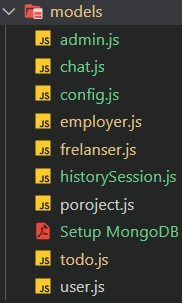
\includegraphics[width=.3\textwidth]{Folders-Files/models.png}
	\centering
	\caption{ساختار پوشه مدل}
	\label{fig:folder-models}
\end{figure}

\subsection{فایل user}
در این فایل به بانک اطلاعات برای ثبت اطلاعات کاربر از جمله مشخصات شناسنامه‌ای، اطلاعات کاربری و رمز و ... پرداخته شده است.

\paragraph{\rl{setUser}:}
ثبت اطلاعات کاربر.
\\
\textbf{توضیحات}
\hr
\begin{flushleft}
	\framebox[.9\textwidth][l]{
		\lr{
			\textcolor{type}{void}
			\textcolor{func}{setUser}
			\textcolor{symb}{(}
			\textcolor{type}{object}
			\textcolor{arg}{newUser}
			\textcolor{symb}{,}
			\textcolor{type}{object}
			\textcolor{arg}{callback}
			\textcolor{symb}{);}
		}
	}
\end{flushleft}
ثبت طلاعات کاربر در بانک اطلاعات.
\\
\textbf{پارامترها}
\hr \\[10pt]
\begin{tabular}{|m{4cm}|m{3cm}|m{10cm}|}
	\hline
	\multicolumn{1}{|c}{پارامتر}
	&
	\multicolumn{1}{|c}{نوع}
	&
	\multicolumn{1}{|c|}{توضیحات}
	\\
	\hline
	\multicolumn{1}{|c}{newUser}
	&
	\multicolumn{1}{|c|}{object}
	&
	0
	\\
	\hline
	\multicolumn{1}{|c}{callback}
	&
	\multicolumn{1}{|c|}{object}
	&
	0
	\\
	\hline
\end{tabular}
\\[10pt]
\textbf{خروجی}
\hr \\
در صورتی که ، در غیر این صورت .


\paragraph{\rl{getUserByEmail}:}
دریافت اطلاعات کاربر با پست الکترونیک.
\\
\textbf{توضیحات}
\hr
\begin{flushleft}
	\framebox[.9\textwidth][l]{
		\lr{
			\textcolor{type}{void}
			\textcolor{func}{getUserByEmail}
			\textcolor{symb}{(}
			\textcolor{type}{string}
			\textcolor{arg}{email}
			\textcolor{symb}{,}
			\textcolor{type}{object}
			\textcolor{arg}{callback}
			\textcolor{symb}{);}
		}
	}
\end{flushleft}
دریافت طلاعات کاربر از بانک اطلاعات توسط پست الکترونیک.
\\
\textbf{پارامترها}
\hr \\[10pt]
\begin{tabular}{|m{4cm}|m{3cm}|m{10cm}|}
	\hline
	\multicolumn{1}{|c}{پارامتر}
	&
	\multicolumn{1}{|c}{نوع}
	&
	\multicolumn{1}{|c|}{توضیحات}
	\\
	\hline
	\multicolumn{1}{|c}{email}
	&
	\multicolumn{1}{|c|}{string}
	&
	0
	\\
	\hline
	\multicolumn{1}{|c}{callback}
	&
	\multicolumn{1}{|c|}{object}
	&
	0
	\\
	\hline
\end{tabular}
\\[10pt]
\textbf{خروجی}
\hr \\
در صورتی که ، در غیر این صورت .


\paragraph{\rl{getUserById}:}
دریافت اطلاعات کاربر با ID.
\\
\textbf{توضیحات}
\hr
\begin{flushleft}
	\framebox[.9\textwidth][l]{
		\lr{
			\textcolor{type}{void}
			\textcolor{func}{getUserById}
			\textcolor{symb}{(}
			\textcolor{type}{int}
			\textcolor{arg}{id}
			\textcolor{symb}{,}
			\textcolor{type}{object}
			\textcolor{arg}{callback}
			\textcolor{symb}{);}
		}
	}
\end{flushleft}
دریافت طلاعات کاربر از بانک اطلاعات توسط ID.
\\
\textbf{پارامترها}
\hr \\[10pt]
\begin{tabular}{|m{4cm}|m{3cm}|m{10cm}|}
	\hline
	\multicolumn{1}{|c}{پارامتر}
	&
	\multicolumn{1}{|c}{نوع}
	&
	\multicolumn{1}{|c|}{توضیحات}
	\\
	\hline
	\multicolumn{1}{|c}{id}
	&
	\multicolumn{1}{|c|}{int}
	&
	0
	\\
	\hline
	\multicolumn{1}{|c}{callback}
	&
	\multicolumn{1}{|c|}{object}
	&
	0
	\\
	\hline
\end{tabular}
\\[10pt]
\textbf{خروجی}
\hr \\
در صورتی که ، در غیر این صورت .

\subsection{فایل employer}
در این فایل به بانک اطلاعات برای اطلاعات داشبورد کارفرما مانند ثبت و بروزرسانی پروژه، دریافت پیشنهادهای انجام پروژه و ... پرداخته شده است.

\subsection{فایل frelanser}
در این فایل به بانک اطلاعات برای ‌اطلاعات داشبورد فریلنسر مانند ثبت رزومه، ثبت پیشنهاد برای انجام پروژه و ... پرداخته شده است.


\section{پوشه مسیر (routes)}
% !TeX root = ../../Report.tex
% !TeX encoding = UTF-8

در این پوشه به تمام مسیر‌های نرم‌افزار پرداخته شده است.
\begin{figure}[H]
	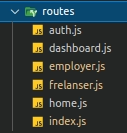
\includegraphics[width=.3\textwidth]{Folders-Files/routes/routes.png}
	\centering
	\caption{ساختار پوشه مسیر}
	\label{fig:folder:routes}
\end{figure}

\subsection{فایل index}
در این فایل مسیرهای برنامه تجمیع شده و تنها این فایل برای دسترسی به مسیرها فراخوانی می‌شود.

\paragraph{\lr{infoApp}:}
شئ حاوی اطلاعات عمومی مانند اطلاعات کاربر، اطلاعات شاخه مسیرها و ... است.

\subsection{فایل home}
در این فایل به مسیرهای صفحه اصلی، لیست کاربران و لیست پروژه‌ها پرداخته شده است.
\paragraph{\lr{CHome}:}
شئ حاوی اطلاعات فایل home در پوشه کنترل‌گر است.

\subsection{فایل auth}
در این فایل به مسیرهای احرازهویت شامل ورود، ثبت‌نام و خروج کاربر پرداخته شده است.

\paragraph{\lr{CAuth}:}
شئ حاوی اطلاعات فایل auth در پوشه کنترل‌گر است.

\subsection{فایل dashboard}
در این فایل به مسیرهای داشبورد کاربر پرداخته شده است.

\paragraph{\lr{CDashboard}:}
شئ حاوی اطلاعات فایل dashboard در پوشه کنترل‌گر است.

\subsection{فایل employer}
در این فایل به مسیرهای داشبورد کارفرما پرداخته شده است.

\paragraph{\lr{CEmployer}:}
شئ حاوی اطلاعات فایل employer در پوشه کنترل‌گر است.

\subsection{فایل frelanser}
در این فایل به مسیرهای داشبورد فریلنسر پرداخته شده است.

\paragraph{\lr{CFrelanser}:}
شئ حاوی اطلاعات فایل frelanser در پوشه کنترل‌گر است.



\section{پوشه نما (views)}
در این پوشه رابط تعامل کاربر با سیستم انجام می‌شود.

\begin{figure}[H]
	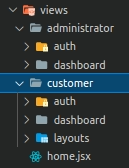
\includegraphics[width=.3\textwidth]{Folders-Files/views.png}
	\centering
	\caption{ساختار پوشه نما}
	\label{fig:folder-views}
\end{figure}


\paragraph{پوشه administrator}
در این پوشه به قالب مدیریت پرداخته شده است.

\subparagraph{پوشه auth}
در این پوشه به قالب احرازهویت مدیریت پرداخته شده است.

\subparagraph{پوشه dashboard}
در این پوشه به قالب داشبورد مدیریت پرداخته شده است.

\subparagraph{پوشه component}
در این پوشه به قالب تکرارشونده مانند منوها، هدر، فوتر و ... پرداخته شده است.


\paragraph{فایل customer}
در این پوشه به قالب کاربر پرداخته شده است.

\subparagraph{پوشه auth}
در این پوشه به قالب احرازهویت کاربر پرداخته شده است.

\subparagraph{فایل login}
در این فایل به قالب ورود کاربر پرداخته شده است.

\subparagraph{فایل signup}
در این فایل به قالب ثبت‌نام کاربر پرداخته شده است.

\subparagraph{پوشه dashboard}
در این پوشه به قالب داشبوردهای کارفرما و فریلنسر پرداخته شده است.

\subparagraph{پوشه component}
در این پوشه به قالب تکرارشونده مانند منوها، هدر، فوتر و ... پرداخته شده است.

\section{پوشه عمومی‌ (public)}
در این پوشه فایل‌های ثابت در کل برنامه مانند تصاویر، css، js و ... قرار می‌گیرد.

\begin{figure}[H]
	%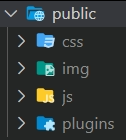
\includegraphics[width=.3\textwidth]{Folders-Files/public.png}
	\centering
	\caption{ساختار پوشه عمومی}
	\label{fig:folder-public}
\end{figure}


\section{فایل اصلی/اجرا (app.js)}
\begin{figure}[H]
	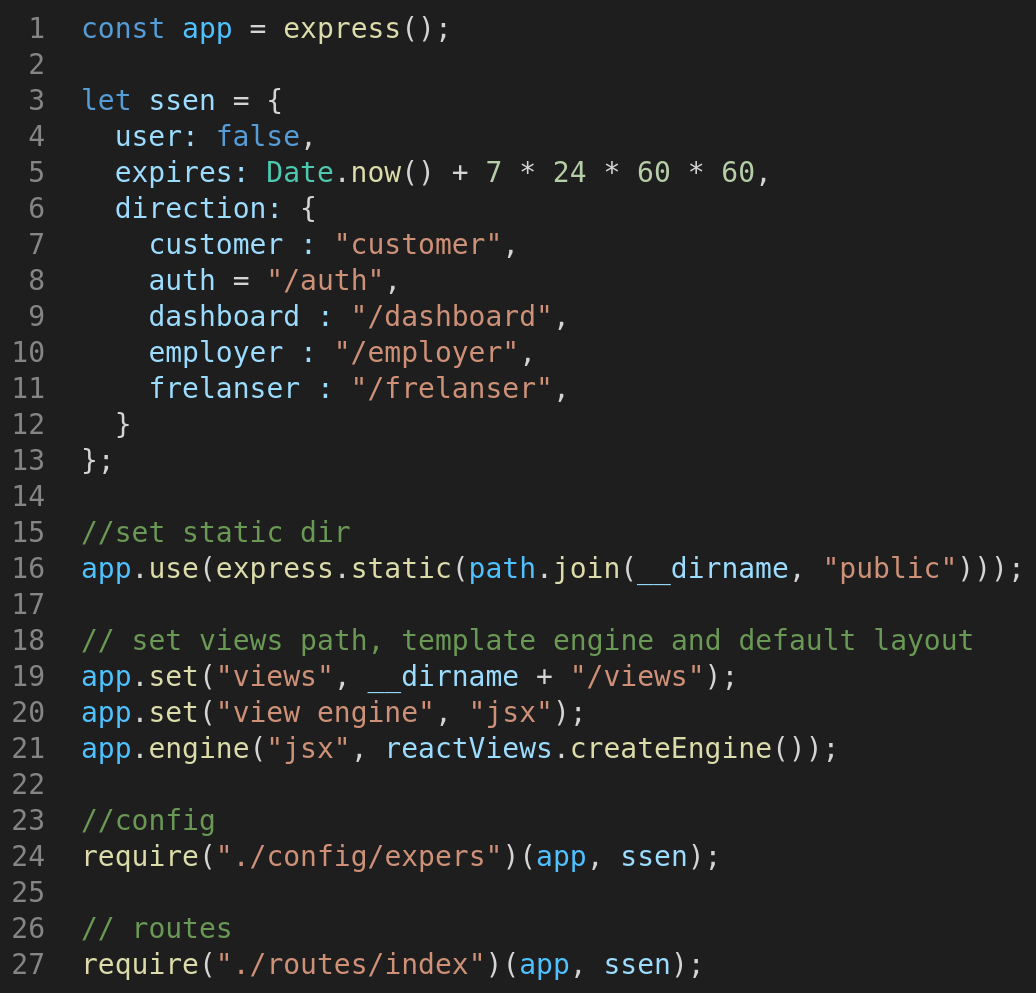
\includegraphics[width=.6\textwidth]{Folders-Files/app.png}
	\centering
	\caption{ساختار فایل frelanser}
	\label{fig:file:routes:frelanser}
\end{figure}

\section{پوشه  (.husky)}
Hook
های لازم جهت مدیریت 
Git
 در این پوشه قرار می‌گیرد.

\section{پوشه  (.vscode)}
 تنظیمات لازم جهت هماهنگی و مدیریت ادیتور 
 \lr{Visual Studio Code}
 در این پوشه قرار می‌گیرد.

\section{پوشه مستندات (docs)}
در این پوشه تمام مستندات برنامه قرار دارد

\begin{figure}[H]
	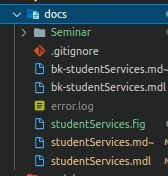
\includegraphics[width=.3\textwidth]{Folders-Files/docs.png}
	\centering
	\caption{ساختار پوشه مستندات}
	\label{fig:folder-docs}
\end{figure}

\paragraph{پوشه Seminar}
در این پوشه اطلاعات سمینار و سمینار تتبع با فرمت و قالب 
 \LaTeX
 قرار دارد.

\section{پوشه گیت‌هاب (.github)}
% !TeX root = ../../Report.tex
% !TeX encoding = UTF-8
در این پوشه تمام اطلاعات گیت‌هاب قرار دارد

\begin{figure}[H]
	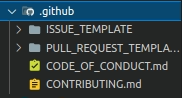
\includegraphics[width=.3\textwidth]{Folders-Files/github.png}
	\centering
	\caption{ساختار قرارگیری گیت‌هاب}
	\label{fig:folder-github}
\end{figure}


\paragraph{پوشه \LR{ISSUE TEMPLATE}}
در این پوشه قالب ایجاد مسئله شامل خطا، باگ و ... در گیت‌هاب قرار دارد.

\paragraph{پوشه \LR{PULL REQUEST TEMPLATE}}
در این پوشه قالب ایجاد درخواست ادغام در گیت‌هاب قرار دارد.

\paragraph{فایل \LR{CODE OF CONDUCT}}
در این فایل نحوه مشارکت در پروژه تعریف شده است.

\paragraph{فایل \LR{CONTRIBUTING}}
در این فایل مشارکت‌کنندگان در پروژه تعریف شده‌اند.


\section{فایل \LR{Environment} (.env)}
% !TeX root = ../../Report.tex
% !TeX encoding = UTF-8
متغیرهای محیطی بخشی اساسی برای توسعه و کار با Node.js یا هر زبان سمت سرور دیگری می باشد. آنها همیشه حاوی داده های بسیار حساس هستند اما با این تفاوت که نمی خواهند داده هایشان را با دنیای بیرون به اشتراک بگذارند.

\section{فایل تاریخچه تغییرات (CHANGELOG)}
% !TeX root = ../../Report.tex
% !TeX encoding = UTF-8
لاگ تغییرات فایلی است که لیست تغییرات قابل توجه برای هر نسخه یک پروژه که بر اساس تاریخ مرتب شدند را شامل می‌شود



\section{فایل \LR{Travis CI} (.travis)}
Travis CI یک سرویس ادغام مداوم توزیع شده و میزبانی شده برای ایجاد و تست پروژه های نرم افزاری میزبانی شده در GitHub می باشد.



\section{فایل \LR{Editor Config} (.editorconfig)}
EditorConfig پلاگینی است که به دولوپرها کمک می‌کند تا بتوانند استایل‌های کدنویسی مد نظر خود را در ادیتورها و محیط‌های توسعهٔ یکپارچه (IDE) مختلف حفظ کنند تا از این طریق پس از سوئیچ کردن بین ادیتورهای مختلف، به‌ خاطر اختلاف فضای محیط کدنویسی، دچار سردرگمی نشوند.

\section{فایل ESLint (.eslintrc)}
% !TeX root = ../../Report.tex
% !TeX encoding = UTF-8
ESLint یک Linter برای زبان برنامه‌نویسی Javascript هست که با استفاده از Node.js به وجود اومده است.

همونطور که میدونین Javascript مانند زبانهای دیگه همچون Java و ... نیست و کامپایلری ندارد و کدها مستقیما در مرورگر اجرا میشن. در زبانهای دیگه که کامپایلر وجود دارد، در زمان compile کردن کد، اگر مشکلی وجود داشته باشد در اکثر موارد بیان میشه و compile با موفقیت به پایان نمیرسه ولی در Javascript به دلیل عدم وجود compiler، مشکلات خودشون رو در زمان اجرا شدن کد در مرورگر نمایش میدن.

ESLint این ارورها رو برای شما پیدا میکنه و جلوی چنین اتفاقاتی رو میگیره. شما بیشتر به دنبال چه نوع ارورهایی هستید که در کدهاتون رخ نده؟
\begin{itemize}
	\item 
	جلوگیری از حلقه‌های بی‌نهایت یا infinite loop با قرار دادن شرط نامناسب
	\item 
	اطمینان از اینکه همه متدهای getter، چیزی رو return میکنند.
	\item 
	جلوگیری از قرار دادن console.log در کدها
	\item 
	چک کردن case‌های تکراری در switch
	\item 
	چک کردن کدهای غیر قابل دسترس. مثلا بعد از return هر کدی رو قرار بدیم، unreachable یا غیر قابل دسترسی میشه.
\end{itemize}

ESLint بسیار منعطف و با قابلیت تنظیم بالا هست. شما میتونین مشخص کنید که چه rule هایی باید برای کدهای شما چک بشه. همچنین میتونین مشخص کنید که چه نوع استایل استانداردی رو میخواید برای کدهاتون قرار بدین. خیلی از rule‌ها بصورت پیش فرض غیر فعال یا فعال هستند و شما میتونین با استفاده از فایل .eslintrc برای کل پروژه‌ها یا یک پروژه خاص، تنظیمات مورد نظرتون رو قرار بدین.

\section{فایل Prettier (.prettierrc)}
Prettier یک ابزار برای شکل‌دهی به کدها است. در واقع این ابزار کاری می‌کند که کدهای شما در یک قالب منحصر به فرد قرار بگیرند و مرتب شوند. 




\section{ساختار پایگاه‌داده}
در این قسمت به ساختار پایگاه داده پرداخته شده است.
\begin{figure}[H]
	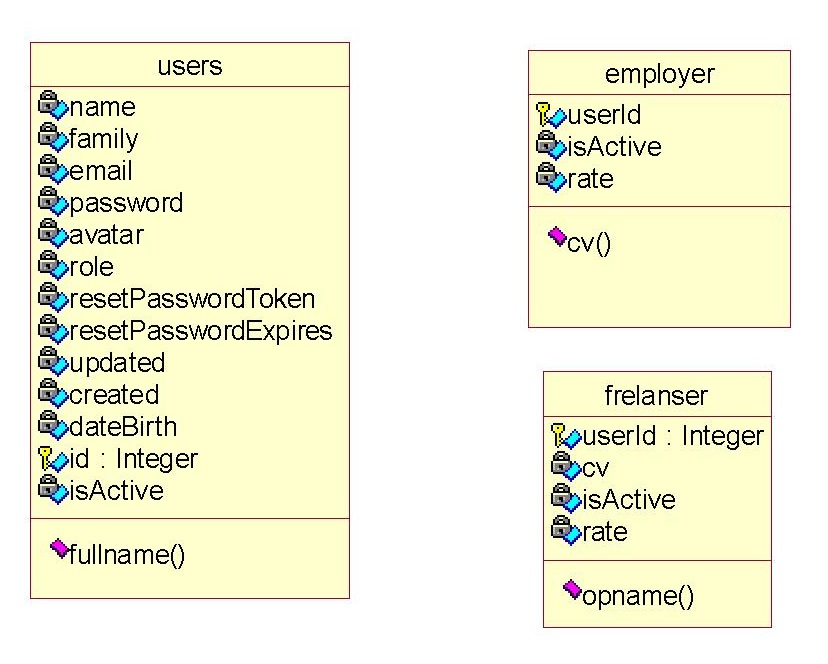
\includegraphics[width=.7\textwidth]{Diagram/6.Class/کلی.jpg}
	\centering
	\caption{ساختار پایگاه داده}
	\label{fig:db:پایگاه}
\end{figure}

\subsection{پایگاه‌داده کاربر}
در این قسمت تمام اطلاعات مربوط به کاربر ثبت می‌شود

\begin{figure}[H]
	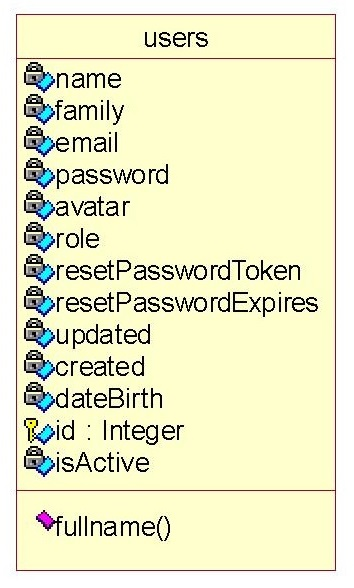
\includegraphics[width=.4\textwidth]{Diagram/6.Class/کاربر.jpg}
	\centering
	\caption{ساختار پایگاه داده کاربر}
	\label{fig:db:کاربر}
\end{figure}


\subsection{پایگاه‌داده کارفرما}
در این قسمت تمام اطلاعات مربوط به ببخش کارفرما ثبت می‌شود.

\begin{figure}[H]
	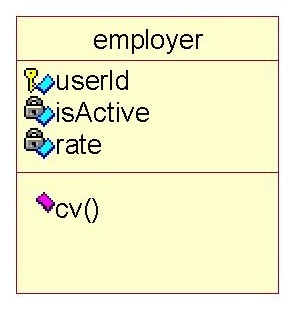
\includegraphics[width=.4\textwidth]{Diagram/6.Class/کارفرما.jpg}
	\centering
	\caption{ساختار پایگاه داده کارفرما}
	\label{fig:db:کارفرما}
\end{figure}

\subsection{پایگاه‌داده فریلنسر}
% !TeX root = ../../Report.tex
% !TeX encoding = UTF-8
در این قسمت تمام اطلاعات مربوط به بخش فریلنسر ثبت می‌شود.

\begin{figure}[H]
	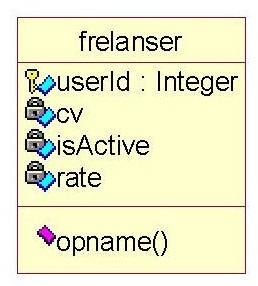
\includegraphics[width=.4\textwidth]{Diagram/6.Class/فریلنسر.jpg}
	\centering
	\caption{ساختار پایگاه داده فریلنسر}
	\label{fig:db:فریلنسر}
\end{figure}

\subsection{پایگاه‌داده مدیریت}
در این قسمت تمام اطلاعات مربوط به بخش مدیریت سایت ثبت می‌شود.

\begin{figure}[H]
	%\includegraphics[width=.4\textwidth]{Diagram/6.Class/مدیریت.jpg}
	\centering
	\caption{ساختار پایگاه داده مدیریت}
	\label{fig:db:مدیریت}
\end{figure}

